\subsection{Testing testing...}

\subsubsection{Testing scenarios}
In order to prepare the WLCG infrastructure for IPv6, the best
approach is to identify beforehand the relevant use cases, starting
from the simplest ones, to take into account the likely constraints
from sites and finally to define realistic scenarios to be used for
testing.

It is reasonable to assume that all central services must work in
dual-stack mode, to be compatible with both IPv4 and IPv6
clients. Site services are strongly encouraged to be run in dual stack
mode as well, lest they incur in limitations (for example in joining
storage federations). On the other hand, clients (including users,
software agents and jobs running on worker nodes) should be able to
exclusively use either protocol, as users may connect from arbitrary
nodes (e.g. their laptop) and worker nodes at some sites might have
only IPv6 public addresses.



This is where the testing results go

some numbers for now: Transfers running since March, some 2.6 million transfers, 86.8 percent success
rate, over 2 PB of data so far. Approx. 7 percent of the rate CMS achieves globally.

The mesh...

\begin{figure}[htp]
\centering
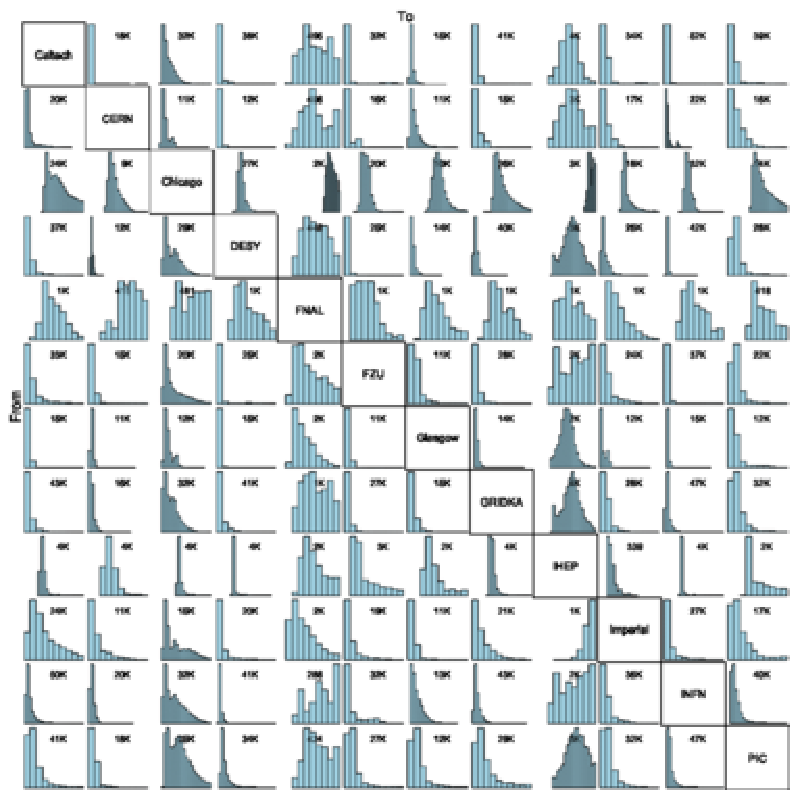
\includegraphics{full-mesh}
\caption{Transfer performance for the IPv6 testbed continuous transfers. A 1 GB file is transferred between each pair of sites, then deleted, then transferred again, continuously. The plots show the distribution of transfer duration times per site pair. The source site is named in the row, the destination site is named in the column. So the top-right plot shows transfers from Caltech to PIC, the bottom-left shows transfers fromPIC to Caltech. The x-axis is in seconds, from 0 to 500 for each plot. The number inset in each plot shows the approximate number of transfers between that site pair in that direction.}\label{fig:full-mesh}
\end{figure}


